\documentclass{jepcs}
\usepackage{graphicx}
\usepackage{booktabs}
\usepackage{tabularx}
\usepackage{array}
\usepackage{hyperref}
\usepackage{fancyhdr}
\hypersetup{pdftitle={Process-Interruption Recovery and Performance Trade-offs in Three Game Save-File Update Strategies: A Reproducible Case Study},pdfauthor={Zain Alaabdin Kassem},pdfsubject={JEPCS Short Communication author manuscript},pdfkeywords={game save systems, crash recovery, fault injection, reproducible benchmarking}}

\fancypagestyle{jepcsfirstpage}{
  \fancyhf{}
  \fancyfoot[L]{\parbox[b]{0.87\textwidth}{\scriptsize Author manuscript; not peer reviewed. \copyright~2026 Zain Alaabdin Kassem. \href{https://github.com/zekk01/game-save-study}{Public study repository}.}}
  \fancyfoot[R]{\scriptsize\thepage}
  \renewcommand{\headrulewidth}{0pt}
}
\jepcsarticletype{Short Communication}
\title{Process-Interruption Recovery and Performance Trade-offs in Three Game Save-File Update Strategies: A Reproducible Case Study}
\author{Zain Alaabdin Kassem}
\jepcsaffiliations{Independent researcher, Dubai, United Arab Emirates}
\jepcscorresponding{zainkassem7@gmail.com}
% Author-copy layout: omit editorial production fields that are assigned only after acceptance.
\fancypagestyle{jepcs}{%
  \fancyhf{}
  \fancyhead[C]{\fontsize{10pt}{10pt}\selectfont\itshape Author manuscript | JEPCS submission}
  \renewcommand{\headrulewidth}{0.5pt}
  \fancyfoot[C]{\fontsize{8pt}{8pt}\selectfont\itshape Page \thepage}
  \renewcommand{\footrulewidth}{0pt}
}
\fancypagestyle{jepcsfirst}{%
  \fancyhf{}
  \fancyfoot[C]{\fontsize{8pt}{8pt}\selectfont Page \thepage}
  \renewcommand{\footrulewidth}{0pt}
}
\renewcommand{\makejepcstitle}{%
  \thispagestyle{jepcsfirst}%
  {\centering
    \includegraphics[width=3.79555in]{\JEPCSLogo}\par
    \vspace{2pt}
    {\bfseries\fontsize{10.5pt}{10.5pt}\selectfont Journal of Emerging Paradigms in Computing Systems (JEPCS) | Author Manuscript\par}%
  }%
  \vspace{-1.5pt}\noindent\rule{\textwidth}{1.1pt}\par
  \vspace{3.5pt}
  {\centering\fontsize{10.5pt}{10.5pt}\selectfont\textbf{ARTICLE TYPE:} \JEPCSArticleType\par}
  \vspace{8pt}
  {\centering
    {\bfseries\fontsize{16pt}{16pt}\selectfont \JEPCSTitle\par}
    \vspace{2pt}
    {\bfseries\fontsize{10.5pt}{10.5pt}\selectfont \JEPCSAuthors\par}
    {\fontsize{9.5pt}{9.5pt}\selectfont \JEPCSAffiliations\par}
    {\fontsize{9.5pt}{9.5pt}\selectfont Corresponding author: \href{mailto:\JEPCSCorresponding}{\JEPCSCorresponding}\par}
  }%
  \vspace{12pt}
}
\begin{document}
\makejepcstitle
\thispagestyle{jepcsfirstpage}

\jepcsabstract{Local game saves can be left incomplete when a game process stops during an update. We compare direct overwrite, same-directory temporary-file replacement, and two-slot generation with SHA-256 validation using synthetic game-state payloads. A .NET harness and a separate Unity 6.3 Windows Player were interrupted at predeclared checkpoints on one Windows 11 workstation. Across three payload sizes, the .NET run recorded 3,500 fault observations and 900 timings; the Unity replication recorded 2,940 fault trials and 900 timings. All 20 trials in each checkpoint group agreed: overwrite had no valid save after truncation until the new payload was complete, while replacement and two-slot retained the old state until commit. No valid trial produced an unexpected state. Median save times ranged from 0.120–0.236 ms, 1.639–5.621 ms, and 0.251–0.632 ms across the three .NET procedures; Unity showed the same recovery pattern, with platform-specific costs. This bounded, reproducible comparison concerns application-process termination only and establishes neither power-loss durability nor cross-platform guarantees.}
\jepcskeywords{Game save systems; crash recovery; file update strategy; fault injection; reproducible benchmarking}

\section{1. Introduction}
Games save progress, inventory, quests, and other world state as a player advances. If the game process stops during a write, the active save may be incomplete. Developers can overwrite that file directly, write a temporary file and replace it, or keep two generations and validate them during recovery. Each option has different costs in write time and storage, and may leave a different state available after an interruption.

Systems research has shown that recovery depends on both application logic and file-system behavior. Pillai et al. found that crash-consistency protocols can rely on file-system properties that vary across systems [1]. Bornholt et al. formalized file-system crash behavior and showed why possible post-crash states need to be considered explicitly [2]. These results also make clear that stopping an application process is a narrower failure model than an operating-system crash or power loss. We use that narrower model here to compare three practical save procedures at controlled points in an update.

We compare the three procedures on one Windows/NTFS system with identical synthetic game-state payloads. The study asks three questions: at which save stages does recovery return the old state, the new state, or no valid state; how do normal save latency and storage use differ; and how does recovery time change with payload size? We provide the protocol, harness, checkpoint results, and measurements so that others can reproduce this specific comparison. The source and data are available in the \href{https://github.com/zekk01/game-save-study}{public study repository}. The procedures themselves are established techniques; our results describe their behavior in this setup, not a new recovery algorithm or a general durability guarantee.

\section{2. Related Work}

Crash-consistency research studies whether application state survives interruptions during storage updates. Pillai et al. examined application protocols and their dependence on file-system persistence properties [1]. Bornholt et al. modeled file-system crash behavior and analyzed temporary-file replacement: on some systems, a rename can persist before the new file's data, leaving an empty or partial file [2]. Temporary-file replacement alone therefore does not guarantee recovery after power loss. Min et al. evaluated an application interface backed by transactional flash storage [3], while Hu et al. examined transactions across storage abstractions [4]. These studies consider failure modes beyond this experiment. We terminate only the writer process at known application checkpoints; we do not test kernel or device failures or infer the order in which data reaches persistent media.

Game-development materials describe save patterns used in practice. PlayFab recommends double-buffering local save files and separately documents cloud conflict handling and rollback [5,6]. Microsoft documents the behavior and platform constraints of .NET's \texttt{File.Replace} method [7]; Microsoft GDK describes temporary-file replacement as a safe-write pattern [8]. These sources guide implementation, but do not evaluate the interruption outcomes measured here. Whittaker compared XML and binary game-data formats by save/load time and file size [9]. Godot's documentation describes JSON save/load and discusses binary serialization [10]. Viotti and Kinderkhedia benchmarked JSON-compatible binary serializers [11]. These works compare persistence formats or performance; they do not test recovery after stopping a game process during an update.

Several studies examine persistence and recovery for online games. Vaz Salles et al. evaluated checkpoint recovery for massively multiplayer online games, including copy-on-update and double-backup approaches in a prototype server [12]. Their system recovers after a server crash through checkpointing and log replay. Cao et al. later proposed checkpoint recovery algorithms for frequently consistent applications, using MMOs as a motivating workload [13]. Zhang's thesis implemented an MMO persistence architecture in the Mammoth framework [14], and Zhang and Kemme measured the performance of transaction consistency models for MMOGs [15]. Knemeyer et al. studied database-backed persistence for distributed real-time applications, including MMOGs [16]. This work addresses server-side state and transactions. Our experiment instead examines local save files after controlled termination of a game process.

The closest methodological comparison we found is Jeon's 2025 preprint on checkpointing for AI training on macOS/APFS [17]. It also injects process crashes at checkpoint phases and measures integrity and write costs, but studies a different domain, platform, and set of update procedures. Mustonen's Unity mobile-game thesis describes a protobuf-net save/load implementation without testing interruption recovery [18].

This is a case study of three local-file implementations under application-process termination, using a synthetic workload on one Windows system. It does not propose a new save method or make a general claim about game-state recovery. The literature search was targeted rather than systematic; its queries and screened sources are recorded in the project repository. The study therefore makes no priority claim, and its findings should be read as specific to the tested procedures and setup.

\section{3. Materials and Methods}
\subsection{3.1. Save procedures}
All strategies began with the same compact UTF-8 JSON payload generated with identical .NET serializer settings. The synthetic state contained player progress, inventory, quest state, and discovered locations. Three procedures were implemented:
\begin{enumerate}
\item \textbf{Direct overwrite}: truncate the active file and write the new serialized payload in 4,096-byte chunks.
\item \textbf{Temporary-file replacement}: create a same-directory temporary file, write and close the new payload, then replace the active file using .NET \texttt{File.Replace}.
\item \textbf{Two-slot generation}: preserve the prior slot and write the next generation to the alternate slot. Each slot stores a generation number, payload, and SHA-256 checksum. Recovery validates each slot and selects the highest-generation valid slot.
\end{enumerate}
The implementation records its checkpoints and API operations. Replacement behavior is evaluated only on this system; no portable atomicity guarantee is assumed.

\subsection{3.2. Workload and failure injection}
Workloads contained 25, 250, or 1,000 items/locations; the quest count was the greater of one and the integer quotient of item count divided by five. Fixed seeds 7 and 19 generated the old and new states. Within a size, all three strategies used the same expected old/new payloads and hashes. The observed payload sizes were 3,025, 29,510, and 117,963 bytes.

The writer ran as a child process and paused at selected checkpoints before destructive operations, after truncation or slot/temp creation, after each write chunk, after close, and around replacement where applicable. The controller terminated the child at the acknowledged checkpoint. Each strategy/size/checkpoint group was repeated 20 times. After termination, the recovery routine classified the result as old-valid, new-valid, no-valid-save, unexpected-state, or recovery-error. A valid result had to match the expected payload hash and state invariants.

At chunk boundaries the writer called \texttt{FileStream.Flush()}, then paused for the controller. This flush moves buffered stream data through the file API, but the study did not request a durable-media flush. The termination mechanism stopped the application process only. The study did not test operating-system crashes, abrupt power loss, storage-controller caches, or physical media failures.

\subsection{3.3. Measurements and analysis}
The fault matrix contained 3 strategies x 3 payload sizes x the applicable predeclared checkpoints x 20 repetitions (3,500 recorded observations overall). Recovery latency measured only the recovery routine and excluded launching the recovery process. Storage bytes recorded the files present after the interruption/recovery path. Normal-save latency used pre-serialized payloads: 10 warm-up saves followed by 100 measurements per strategy and payload size. Timing included file writes, stream flushes, replacement or checksum/envelope work, as applicable; payload generation and JSON serialization were excluded. Strategy order was shuffled with a fixed seed per size.

We report medians and interquartile ranges (IQR) for save latency because the distributions included outliers. Paired median differences compare temporary-file replacement with direct overwrite using 10,000 bootstrap resamples of matched timing observations and a fixed resampling seed. These intervals describe resampling variability within this run only; they are not population intervals over devices, players, or systems. Fault-trial counts are repeated observations at selected checkpoints, not estimates of real-world crash probabilities.

\subsection{3.4. Unity runtime replication}
A separate replication used Unity 6000.3.11f1 and its standalone Windows Player, built-in \texttt{JsonUtility} serializer, and \texttt{Application.persistentDataPath}. It implemented the same three procedures and workload sizes, with the same deterministic seeds and 4,096-byte chunks; checkpoints followed stream flushes and the controller terminated the Player process after acknowledgment. Unity payloads were 3,027, 29,523, and 118,027 bytes. This matrix contained 147 size/strategy/checkpoint groups with 20 repetitions each, and a separate 900-row timing run with 10 warm-ups and 100 measurements per strategy and size. Recovery used exact Unity-generated payload hashes and state invariants. Four initial 25-item/direct trial directories collided with excluded pilot smoke data because of a controller path bug. The four rows remain visible as controller errors; each was replaced by a new trial 21, yielding 20 valid main trials in each group. Unity files were under C: (WD PC SN560), whereas the .NET main run used D: (Intel SSDPEKNU512GZ); results are analyzed separately and not pooled.

\section{4. Experimental Setup}
The .NET main experiment used a standalone C\# console harness. It ran in Release configuration on Windows 11 IoT Enterprise LTSC, build 26100 (64-bit), using .NET runtime 9.0.6 and SDK 9.0.301. The processor was an AMD Ryzen 9 7845HX (12 cores/24 logical processors). Save and result files resided on D:, a local NTFS volume on an Intel SSDPEKNU512GZ NVMe drive (nominal 512 GB). The separate Unity runtime replication used Unity 6000.3.11f1 and wrote saves to C:, a local NTFS volume on a WD PC SN560 NVMe drive (nominal 1 TB). Both runs used the same workstation; because their save volumes differed, their timing values are not direct runtime comparisons. The power plan observed after the runs was Balanced; AC/battery state during data collection was not recorded. The .NET primary data comprise 3,500 fault trials and 900 timing rows; the Unity replication comprises 2,940 valid fault trials, four preserved controller-error rows, and 900 timing rows.

The .NET metadata file labels the protocol as \texttt{protocol-v1-draft}, due to a stale metadata constant. Run parameters match protocol version 1, and the discrepancy is documented in the run context; original metadata was not edited. The .NET audit verified expected row/group counts, no duplicates or incomplete groups, and no inconsistent payload hashes or sizes. The Unity audit separately verified 147 complete groups of 20 valid main trials and 900 timing rows; the four pilot-collision records remain in the raw CSV and are excluded from main-trial counts. These audits are data-integrity checks, not independent validation of the experimental design.

\section{5. Results and Discussion}
\subsection{5.1. Recovery outcomes}
Across 3,500 interruption observations, recovery returned the old valid state 2,440 times, the new valid state 300 times, and no valid save 760 times. There were no unexpected states or recovery errors. These counts aggregate different checkpoints and strategies and must not be interpreted as crash likelihoods.

For direct overwrite, all repetitions before truncation recovered the old state. Following truncation, the old file was no longer valid; partial writes remained invalid until the complete new payload was present. For temporary-file replacement, the original save remained valid while the separate temporary file was written; recovery selected the new state after replacement. For two-slot saves, the old generation remained available while the alternate slot was incomplete; after a complete checksummed envelope was available, recovery selected the new generation. All 20 repetitions within each tested checkpoint group had the same outcome. This agreement reflects deterministic, controlled checkpoints on one system, not exhaustive fault coverage.

\subsection{5.2. Normal save latency and storage}
Table~\ref{tab:timings} shows that direct overwrite had the lowest median latency in this run at each payload size. Temporary-file replacement showed a median of 1.639--5.621 ms, while direct overwrite ranged from 0.120--0.236 ms. The two-slot method ranged from 0.251--0.632 ms. The relative ordering and timings are specific to the implementation, runtime, Windows/NTFS stack, and device; no claim is made that the same ranking holds elsewhere.

The paired median latency difference (replacement minus direct) was 1.507 ms (95\% paired bootstrap interval 1.474--1.538) for 25 items, 5.030 ms (4.846--5.197) for 250, and 5.174 ms (4.912--5.363) for 1,000. Intervals quantify uncertainty under resampling of these observed pairs only. The two-slot normal-save directory occupied 10,810, 103,380, and 412,286 bytes at the three sizes, respectively, approximately 3.50--3.57 times the base payload. Direct overwrite and replacement occupied approximately one payload equivalent in their normal-save directories. Figure~\ref{fig:latency} shows the timing distributions and their outliers; Figure~\ref{fig:storage} compares directory footprint with base payload size. The two-slot footprint is the expected storage cost of retaining two encoded slots and metadata, measured here rather than assumed.

\begin{table}[t]
\centering
\caption{Normal save latency (median, IQR) and post-save directory footprint. Latency values are milliseconds; footprint is bytes.}
\label{tab:timings}
\renewcommand{\arraystretch}{1.15}
\setlength{\tabcolsep}{3pt}
\begin{tabularx}{\textwidth}{@{}rX X X r@{}}
\toprule
\textbf{Items} & \textbf{Direct overwrite} & \textbf{Temp + replace} & \textbf{Two-slot + checksum} & \textbf{Payload (B)}\\
\midrule
25 & 0.120 (0.112--0.132); 3,025 B & 1.639 (1.565--1.742); 3,025 B & 0.632 (0.161--1.362); 10,810 B & 3,025\\
250 & 0.156 (0.146--0.232); 29,510 B & 5.391 (4.999--5.923); 29,510 B & 0.251 (0.238--0.279); 103,380 B & 29,510\\
1,000 & 0.236 (0.227--0.353); 117,963 B & 5.621 (5.186--5.912); 117,963 B & 0.536 (0.521--0.582); 412,286 B & 117,963\\
\bottomrule
\end{tabularx}
\end{table}

\begin{figure}[t]
\centering
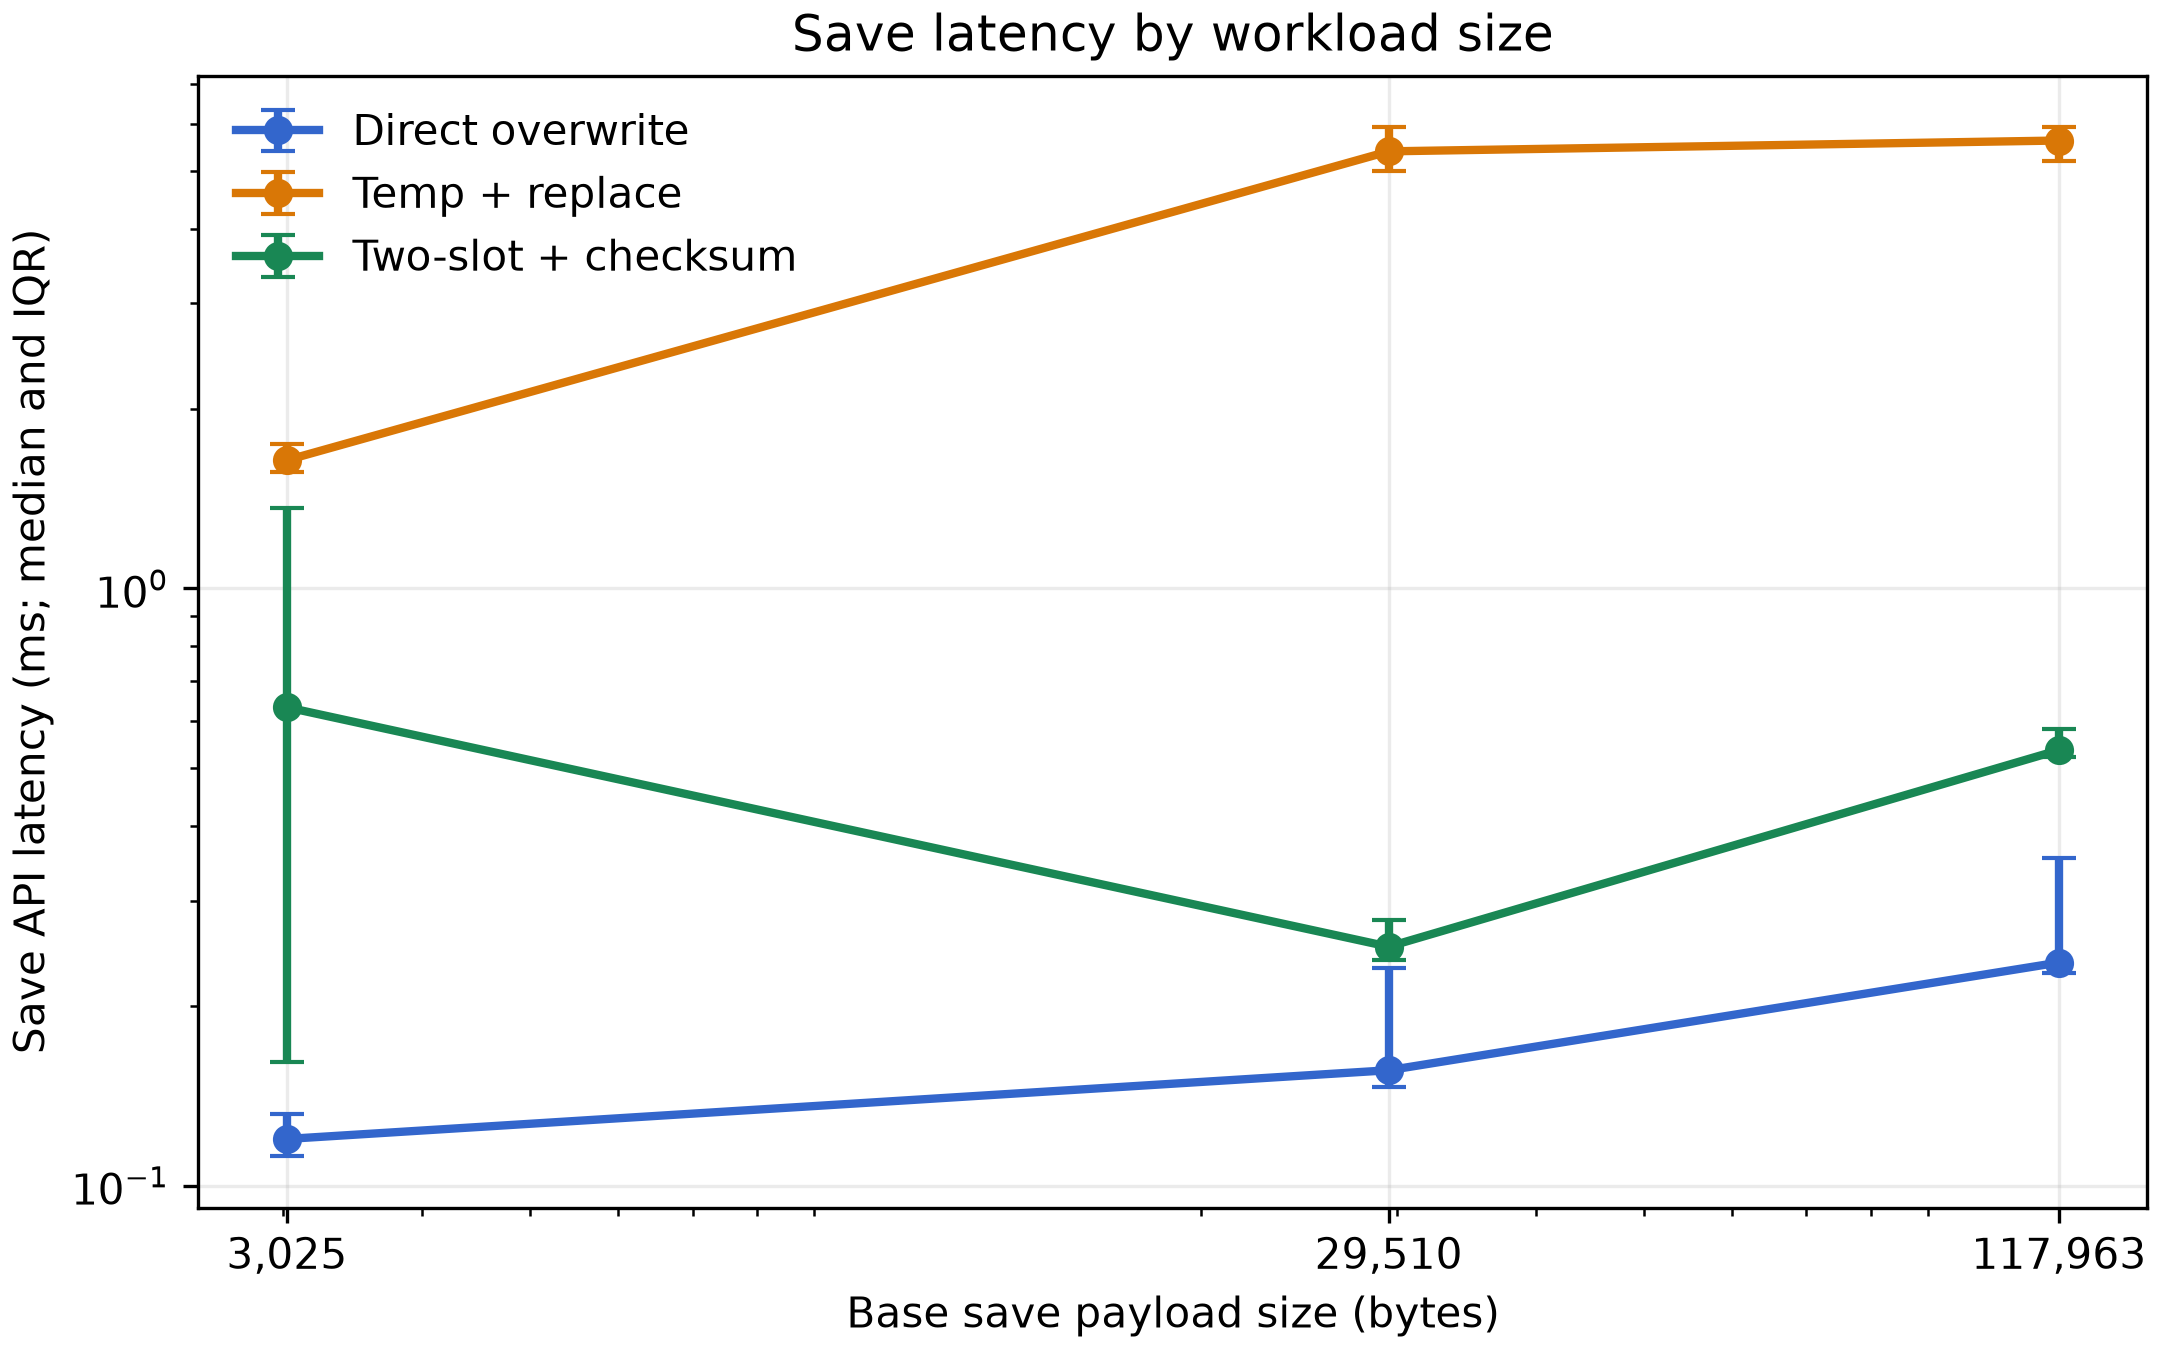
\includegraphics[width=0.96\textwidth]{figure-latency.png}
\caption{Normal save latency by payload size and update procedure. Points/distribution summaries reflect 100 measurements per group; the plot shows the observed variability and outliers.}
\label{fig:latency}
\end{figure}

\begin{figure}[t]
\centering
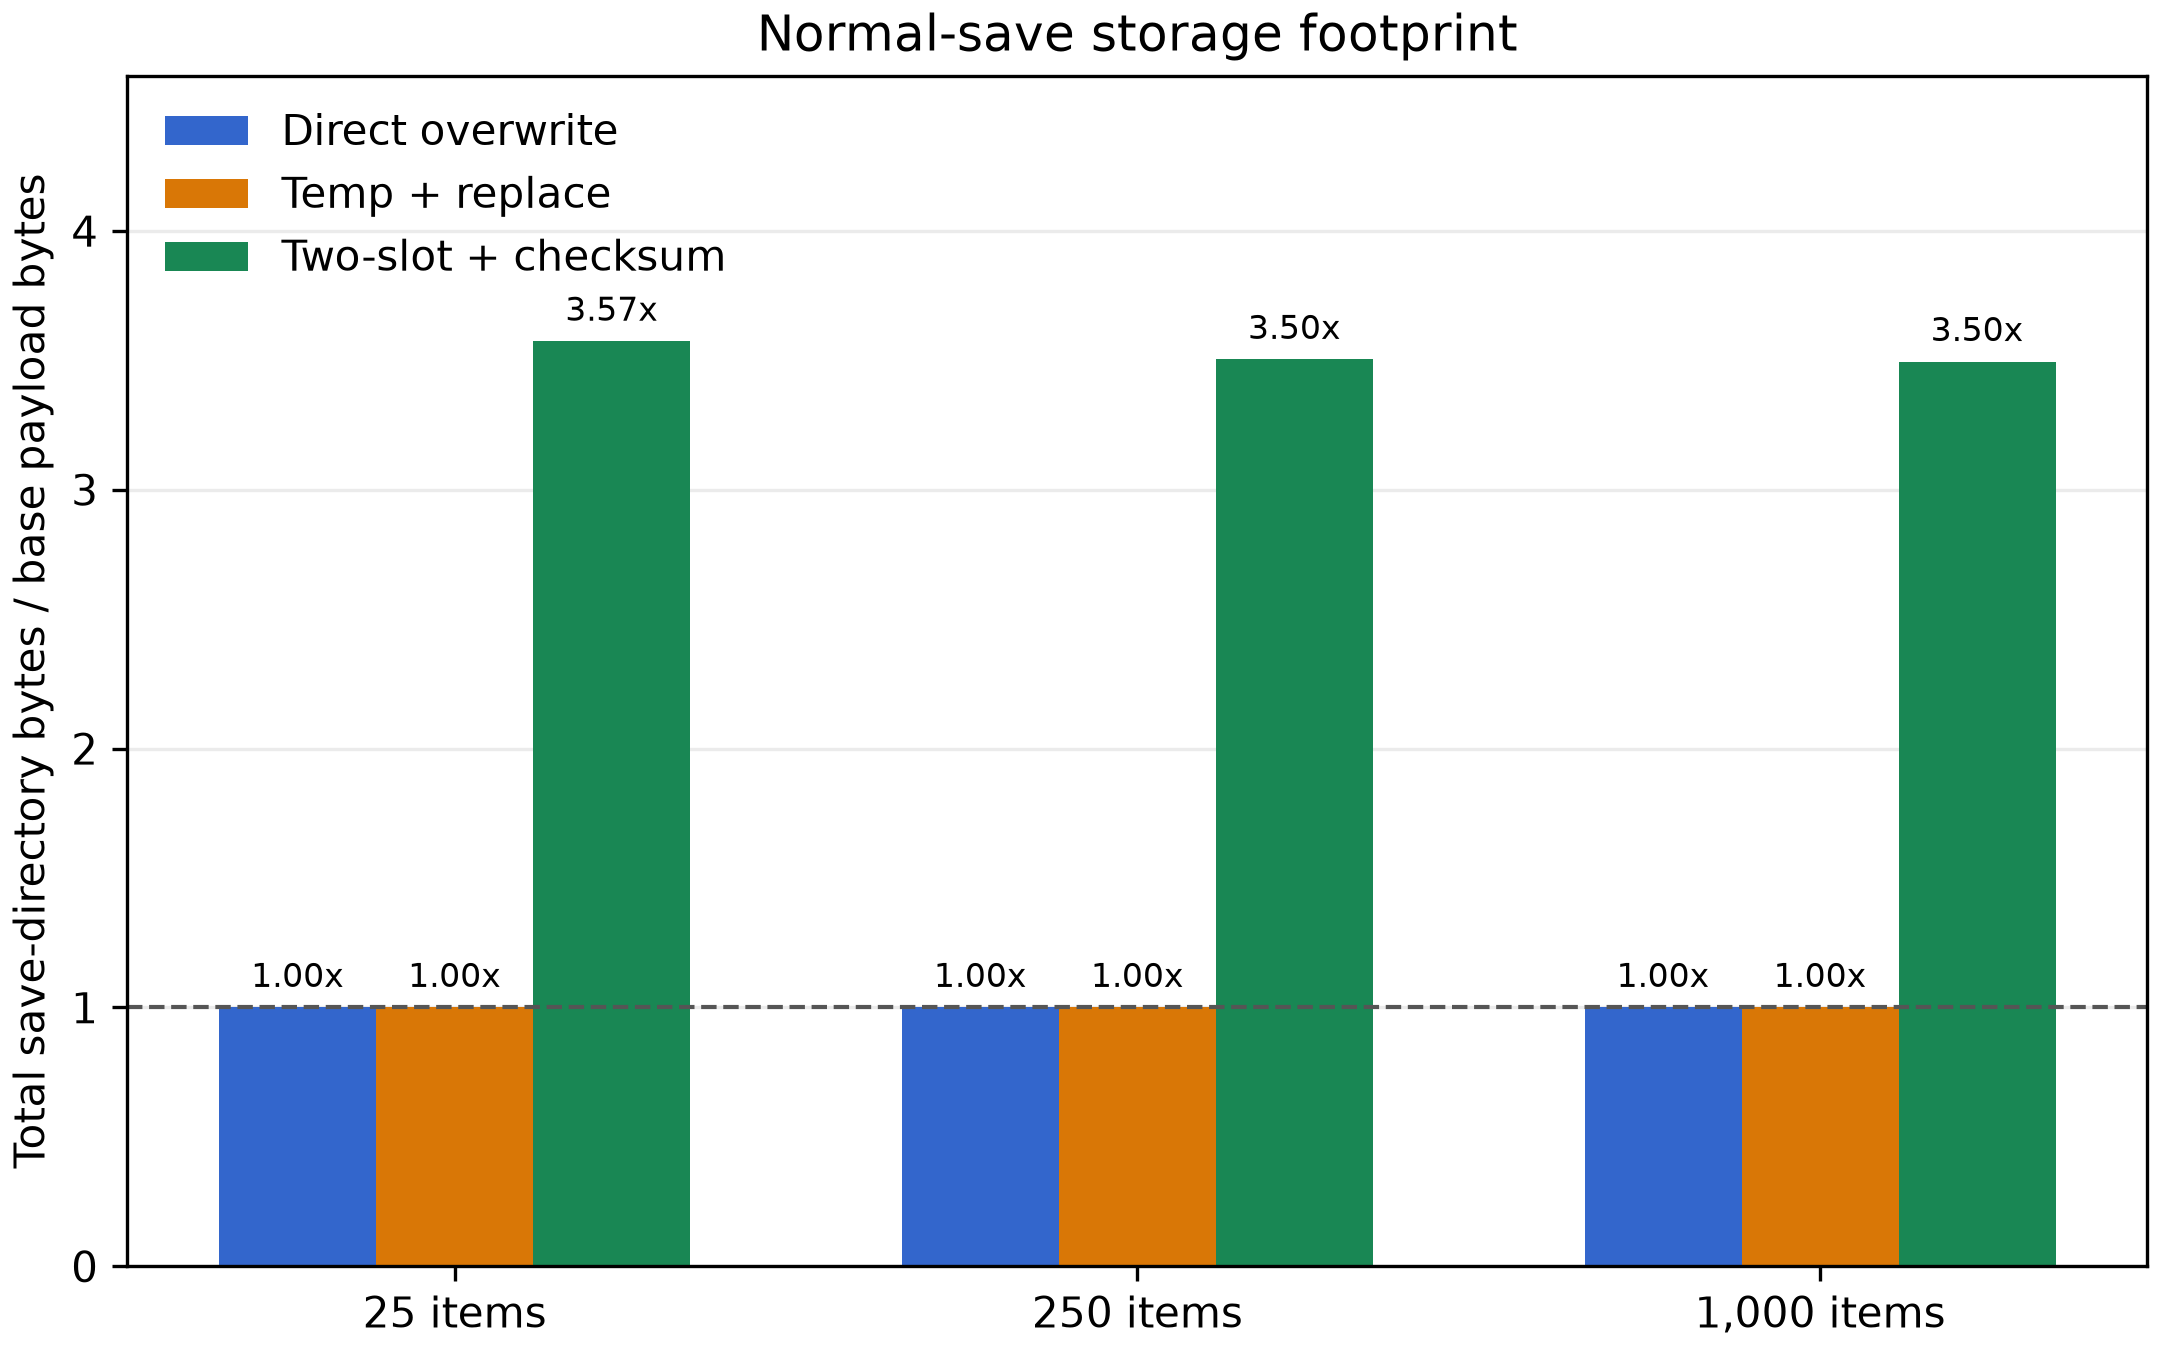
\includegraphics[width=0.90\textwidth]{figure-storage.png}
\caption{Normal-save directory footprint relative to the serialized payload size. Two-slot storage retains additional encoded state to preserve a previous generation.}
\label{fig:storage}
\end{figure}

\subsection{5.3. Recovery routine latency}
Median recovery routine time rose with workload size for every strategy. For 25 items, medians were 0.164 ms (direct), 0.150 ms (replacement), and 0.307 ms (two-slot). For 250 items, they were 0.300, 0.288, and 0.763 ms; for 1,000 items, 0.643, 0.781, and 1.511 ms, respectively. These are descriptive measurements across the injected checkpoints. Since checkpoint state and file contents differ, they are not clean isolated estimates of an algorithmic cost, and process startup is excluded.

\subsection{5.4. Unity replication}
The Unity Player produced the same checkpoint-level recovery classification in all 147 groups: across 2,940 valid main trials, 1,880 recovered the old state, 760 had no valid save, and 300 recovered the new state; no trial produced an unexpected state or recovery error. The 25-item/direct pilot collisions are excluded from these counts, with the original four controller-error records preserved and four replacement trials recorded. The pattern matched the .NET study: direct overwrite exposed an invalid-save interval after truncation, while replacement and two-slot retained a valid older state until commit.

Unity median save latencies were 0.142/0.196/0.316 ms for direct overwrite, 1.678/5.787/5.969 ms for replacement, and 0.238/1.093/2.524 ms for two-slot at 25/250/1,000 items, respectively. The two-slot save directory used 7,177/68,100/271,528 bytes, or about 2.3 times the payload; direct and replacement used approximately one payload. These Unity values are a separate within-runtime/device description: Unity wrote to the C: WD volume, whereas .NET wrote to the D: Intel volume, so absolute timings should not be read as an engine-versus-runtime effect. The agreement in recovery outcomes is a same-workstation replication across different serializers and save volumes, not an independent-platform validation.

\subsection{5.5. Practical interpretation and validity}
The results illustrate a familiar trade-off: direct overwrite is fast and space-efficient during normal saves but exposes a period with no valid file after truncation; the other procedures preserve the prior generation during more of the update, at a time or storage cost. Which trade-off is acceptable depends on a game's state value, expected save frequency, platform, and recovery requirements. The experiment does not measure player harm, perceived reliability, or game-engine integration effort.

Several threats limit interpretation. First, both runs used one workstation and operating system; the two different volumes add a storage-device difference, so timing results are not directly comparable between runtimes. Second, controlled application termination is weaker than power loss or kernel failure; stream flushes did not request durable-media synchronization. Third, a synthetic deterministic JSON workload cannot represent all real game states, compression, encryption, asynchronous save pipelines, cloud synchronization, or platform-specific storage APIs. Fourth, each runtime was run once; repeated timings in one run do not replace independent runs or multiple devices. Fifth, results depend on the specific implementations and checkpoint set. Finally, literature searching was targeted rather than systematic, so no exhaustive novelty claim is justified. A stronger follow-up should repeat the protocol across multiple machines and operating systems, add reboot/power-loss testing where safe, and compare additional engine-native save implementations.

\section{6. Conclusion and Future Work}
This case study compared direct overwrite, temporary-file replacement, and two-slot checksummed saves using controlled process termination and a synthetic game-state workload. The .NET study and separate Unity replication showed the same checkpoint-level recovery pattern: direct overwrite temporarily had no valid save after truncation, while the other strategies preserved a prior generation until a new complete state was available. Direct overwrite had the lowest normal-save latency and storage footprint within each run; the two-slot footprint was about 3.5 times the payload in .NET and 2.3 times in Unity. The timing results are specific to separate save volumes and are not a runtime comparison. These are bounded empirical observations, not platform-independent guarantees.

The immediate next step is independent replication on additional devices and operating systems with durable-flush semantics and machine-level fault injection. Further work should include real engine save paths, larger/compressed payloads, and workload patterns from actual games. The study artifacts are publicly available at \href{https://github.com/zekk01/game-save-study}{the project repository}; independent replication and further review are recommended.

\section{Author Declarations}
\jepcsdeclaration{Author Contributions (CRediT)}{Zain Alaabdin Kassem: Conceptualization, Supervision, Validation, Software, Writing -- review \& editing.}
\jepcsdeclaration{Funding}{This research received no external funding; it was self-funded by the author.}
\jepcsdeclaration{Data Availability Statement}{The raw observations, analysis scripts, protocol, manuscript source, and Unity prototype are publicly available at \href{https://github.com/zekk01/game-save-study}{public study repository}. No DOI has been assigned to this repository.}
\jepcsdeclaration{Acknowledgments}{No additional acknowledgments. Generative AI assistance is disclosed separately below.}
\jepcsdeclaration{Conflicts of Interest}{The author declares no competing interests.}
\jepcsdeclaration{Ethics Statement}{Not applicable. No human participants, animals, or personal data were involved.}

\textbf{Declaration of Generative AI:}\par
ChatGPT (OpenAI) assisted with literature searches, coding, data-analysis support, and manuscript drafting. The author critically revised the manuscript, reviewed the prototype code, checked the reported results, and accepts responsibility for the final content.

\section{References}
\begin{jepcsreferences}
\jepcsref{1}{
T. S. Pillai, V. Chidambaram, R. Alagappan, S. Al-Kiswany, A. C. Arpaci-Dusseau, and R. H. Arpaci-Dusseau,
``All File Systems Are Not Created Equal: On the Complexity of Crafting Crash-Consistent Applications,''
in \textit{Proceedings of the 11th USENIX Symposium on Operating Systems Design and Implementation (OSDI)}, Broomfield, CO, USA, 2014, pp. 433--448.
}
\jepcsref{2}{
J. Bornholt, A. Kaufmann, J. Li, A. Krishnamurthy, E. Torlak, and X. Wang,
``Specifying and Checking File System Crash-Consistency Models,''
in \textit{Proceedings of the 21st International Conference on Architectural Support for Programming Languages and Operating Systems (ASPLOS)}, 2016, pp. 83--98, doi: 10.1145/2872362.2872406.
}
\jepcsref{3}{
C. Min, W.-H. Kang, T. Kim, S.-W. Lee, and Y. I. Eom,
``Lightweight Application-Level Crash Consistency on Transactional Flash Storage,''
in \textit{Proceedings of the 2015 USENIX Annual Technical Conference}, Santa Clara, CA, USA, 2015, pp. 221--234.
}
\jepcsref{4}{
Y. Hu, Y. Kwon, V. Chidambaram, and E. Witchel,
``From Crash Consistency to Transactions,''
in \textit{Proceedings of the 16th Workshop on Hot Topics in Operating Systems (HotOS)}, Whistler, BC, Canada, 2017, pp. 100--105, doi: 10.1145/3102980.3102997.
}
\jepcsref{5}{
Microsoft,
``Game Saves overview,''
Microsoft Learn. Accessed: November 2, 2026. [Online]. Available: \url{https://learn.microsoft.com/en-us/xbox/playfab/player-progression/game-saves/overview}.
}
\jepcsref{6}{
Microsoft,
``Game Save conflicts and atomic units,''
Microsoft Learn. Accessed: November 2, 2026. [Online]. Available: \url{https://learn.microsoft.com/en-us/xbox/playfab/player-progression/game-saves/conflicts}.
}
\jepcsref{7}{
Microsoft,
``File.Replace Method (System.IO),''
Microsoft Learn. Accessed: November 2, 2026. [Online]. Available: \url{https://learn.microsoft.com/en-us/dotnet/api/system.io.file.replace?view=net-9.0}.
}
\jepcsref{8}{
Microsoft,
``Game Saves overview,''
Microsoft Game Development Kit documentation. Accessed: November 2, 2026. [Online]. Available: \url{https://learn.microsoft.com/en-us/gaming/gdk/docs/features/common/game-save/game-saves-overview}.
}
\jepcsref{9}{
D. Z. Whittaker,
\textit{Generic Dynamic DataContainer for Rapid Game Development},
M.S. thesis, Department of Computer Science, University of Victoria, Victoria, BC, Canada, 2009. [Online]. Available: \url{https://dspace.library.uvic.ca/server/api/core/bitstreams/01a43792-2af9-49d7-9957-4b520668ca37/content}.
}
\jepcsref{10}{
Godot Engine contributors,
``Saving games,''
Godot Engine documentation, stable version. Accessed: November 2, 2026. [Online]. Available: \url{https://docs.godotengine.org/en/stable/tutorials/io/saving_games.html}.
}
\jepcsref{11}{
J. C. Viotti and M. Kinderkhedia,
``A Benchmark of JSON-compatible Binary Serialization Specifications,''
arXiv:2201.03051, 2022, doi: 10.48550/arXiv.2201.03051.
}
\jepcsref{12}{
M. Vaz Salles, T. Cao, B. Sowell, A. Demers, J. Gehrke, C. Koch, and W. White,
``An Evaluation of Checkpoint Recovery for Massively Multiplayer Online Games,''
\textit{Proceedings of the VLDB Endowment}, vol. 2, no. 1, pp. 1258--1269, 2009, doi: 10.14778/1687627.1687769.
}
\jepcsref{13}{
T. Cao, M. Vaz Salles, B. Sowell, Y. Yue, A. Demers, J. Gehrke, and W. White,
``Fast Checkpoint Recovery Algorithms for Frequently Consistent Applications,''
in \textit{Proceedings of the ACM SIGMOD International Conference on Management of Data}, 2011, pp. 265--276, doi: 10.1145/1989323.1989352.
}
\jepcsref{14}{
K. Zhang,
\textit{Persistent Transaction Models for Massively Multiplayer Online Games},
M.S. thesis, School of Computer Science, McGill University, Montréal, QC, Canada, 2010. [Online]. Available: \url{https://www.collectionscanada.gc.ca/obj/thesescanada/vol2/002/MR72985.PDF}.
}
\jepcsref{15}{
K. Zhang and B. Kemme,
``Transaction Models for Massively Multiplayer Online Games,''
in \textit{Proceedings of the 30th IEEE International Symposium on Reliable Distributed Systems (SRDS)}, 2011, pp. 31--40, doi: 10.1109/SRDS.2011.13.
}
\jepcsref{16}{
M. Knemeyer, A. Ploss, F. Glinka, M. Nsaif, and S. Gorlatch,
``The Problem of Data Persistency in Distributed Real-Time Interactive Applications,''
in \textit{Proceedings of the 2013 IEEE 7th International Conference on Intelligent Data Acquisition and Advanced Computing Systems (IDAACS)}, 2013, pp. 203--207, doi: 10.1109/IDAACS.2013.6662671.
}
\jepcsref{17}{
J. Jeon,
``Crash-Consistent Checkpointing for AI Training on macOS/APFS,''
arXiv:2511.18323, 2025, doi: 10.48550/arXiv.2511.18323. [Online]. Available: \url{https://arxiv.org/abs/2511.18323}. Preprint; not peer reviewed as of the literature search date.
}
\jepcsref{18}{
S.-M. Mustonen,
\textit{Mobile Game Prototype for Savonia},
bachelor's thesis, Savonia University of Applied Sciences, 2015. [Online]. Available: \url{https://www.theseus.fi/bitstream/handle/10024/102084/Mustonen_Sini-Maaret.pdf?sequence=1}.
}
\end{jepcsreferences}

\end{document}
